\chapter{Experimental Setup}
\label{chapter:experiment}

\section{The Large Hadron Collider}
In order to extend the energy frontier for collision experiments, the existing LEP tunnel was repurposed to house a new proton-proton machine, the Large Hadron Collider (LHC).  The \SI{26.7}{km} LEP ring consists of eight straight sections connected by eight arcs, housed at a depth of \SIrange{45}{170}{m} beneath farmland surrounding the Franco-Swiss border~\cite{Evans:1129806}.  The LHC is now the most powerful collider in the world, currently operating at a center-of-mass energy of \SI{8}{\TeV}, although this thesis considers only the 2011 runs at the slightly lower energy of \SI{7}{\TeV}.  The LHC operators plan to nearly double the collision energy by 2015.

Although a proton is nominally composed of only three quarks, its structure also involves gluons and $q\bar{q}$ pairs in continual flux.  Each of these constituents, including the short-lived components of the proton ``sea'', carries some fraction of the proton's overall momentum.  While the three valence quarks typically carry the largest portions, the antiquarks in the sea have some probability to fluctuate to comparable momenta.  Many previous hadron colliders have followed a $p\bar{p}$ design in order to maximize the possibility of high-energy valence $q\bar{q}$ interactions which have the possibility of generating a wide range of colorless final states.  The difficulty of producing antiprotons in large numbers, however, limits the achievable luminosity of such machines.  The $pp$ design of the LHC will allow it to attain luminosities many orders of magnitude beyond those seen at the Tevatron.  

The instantaneous luminosity for a symmetric colliding beam experiment such as the LHC is given as:
\begin{equation}
  \label{eq:luminosity}
  \mathcal{L} = \frac{n N^2 f}{A_\text{eff}}
\end{equation}
with $n$ the number of bunches per beam, $N$ the number of particles per bunch, $f$ the revolution frequency (\SI{11.246}{kHz}), and $A_\text{eff}$ the effective cross-sectional area of the beams.  The beams are focused to \SI{16}{\micro m} in each of the transverse directions ($\sigma_x$ and $\sigma_y$) which can be used to calculate the value of $A_\text{eff} = 4\pi \sigma_x \sigma_y$. The values of $n$ and $N$ have changed as the luminosity has progressed, so values are given by machine era in Table~\ref{tab:lhcparameters} while the total integrated luminosity delivered over the course of 2011 can be seen in Figure~\ref{fig:lumivstime}.

% The achieved luminosity is determined by various parameters of the beam as:
% \begin{equation}
%   \label{eq:luminosity}
%   \mathcal{L} = \frac{k N^2 f}{4\pi \sigma_x^{*} \sigma_y^{*}}
% \end{equation}
% where $k$ is the number of bunches per beam, $N$ is number of particles per bunch, $f$ is the revolution frequency (\SI{11.246}{kHz}), and $\sigma^{*}$ is the size of the beam at the collision point ($\sigma_x^{*} = \sigma_y^{*}$ = \SI{16}{\micro m}).  The values of these various parameters for given running periods are given in Table~\ref{tab:lhcparameters}.

\begin{table*}
  \centering
  \newcommand{\phan}{\phantom{0}}
  \begin{tabular}{l c c r c c}
    %http://lhc-commissioning.web.cern.ch/lhc-commissioning/
    \toprule
    Era & $E/\TeV$ & $\sqrt{s}/\TeV$ & $\mathcal{L}/(\si{cm^{-2}s^{-1}})$ & $N$ & $n$ \\
    \midrule
    Late \hfill 2010 & 3.5 & \phan 7 & \num{  2e32} & \num{e11} & \phan 348 \\
    Early       2011 & 3.5 & \phan 7 & \num{ 10e32} & \num{e11} & \phan 874 \\
    Late \hfill 2011 & 3.5 & \phan 7 & \num{ 30e32} & \num{e11} & 1318 \\
    Early       2012 & 4.0 & \phan 8 & \num{ 60e32} & \num{e11} & 1318 \\
    Design           & 7.0 &      14 & \num{100e32} & \num{e11} & 2835 \\
    \bottomrule
  \end{tabular}
  \caption[LHC operation parameters]{LHC operation parameters where $E$ is beam energy, $\sqrt{s}$ is center of mass energy, $\mathcal{L}$ is instantaneous luminosity, $N$ is the number of protons per bunch, and $n$ is the number of bunches per beam.  These numbers are only approximate, as the real luminosity progression has occurred in much smaller steps, with frequent tests of new configurations.}
  \label{tab:lhcparameters}
\end{table*}

\begin{figure*}
  \centering
  \includegraphics[width=\plotwidth]{matplotlib/lumivstime}
  \caption[Integrated luminosity recorded by the CMS detector vs.~time]{The integrated luminosity both \emph{delivered} by the LHC to CMS and \emph{recorded} by CMS in 2011.  The difference between delivered and recorded luminosities corresponds to a downtime less than 10\% for the CMS detector during the 2011 runs.}
  \label{fig:lumivstime}
\end{figure*}

The CERN accelerator complex includes a series of components which progressively accelerate the proton beams to higher energies.
The LHC makes use of the LEP injection chain to accelerate the protons to an energy of \SI{450}{\GeV} before entering the main ring.  
The first stage uses the Linac2 to boost the protons to \SI{50}{\MeV} in a series of radio frequency (RF) cavities, followed by similar pushes in the Proton Synchrotron Booster (PSB) to \SI{1.4}{\GeV} and then the Proton Synchrotron (PS) to \SI{24}{\GeV}.  In the PSB, magnets begin focusing the beam while its bunch structure is introduced in several steps through the PSB and PS stages.  The protons are brought up to a full injection energy of \sienergy{450} in the Super Proton Synchrotron (SPS).  Before taking on its current role as the main LHC injector, the SPS served as the colliding machine for its own round of new physics discoveries, delivering beam to the UA1 and UA2 experiments which first confirmed the existence of the $W$ and $Z$ bosons.  A schematic of these accelerator stages is available in Figure~\ref{fig:lhc-complex}.

\begin{figure*}
  \centering
  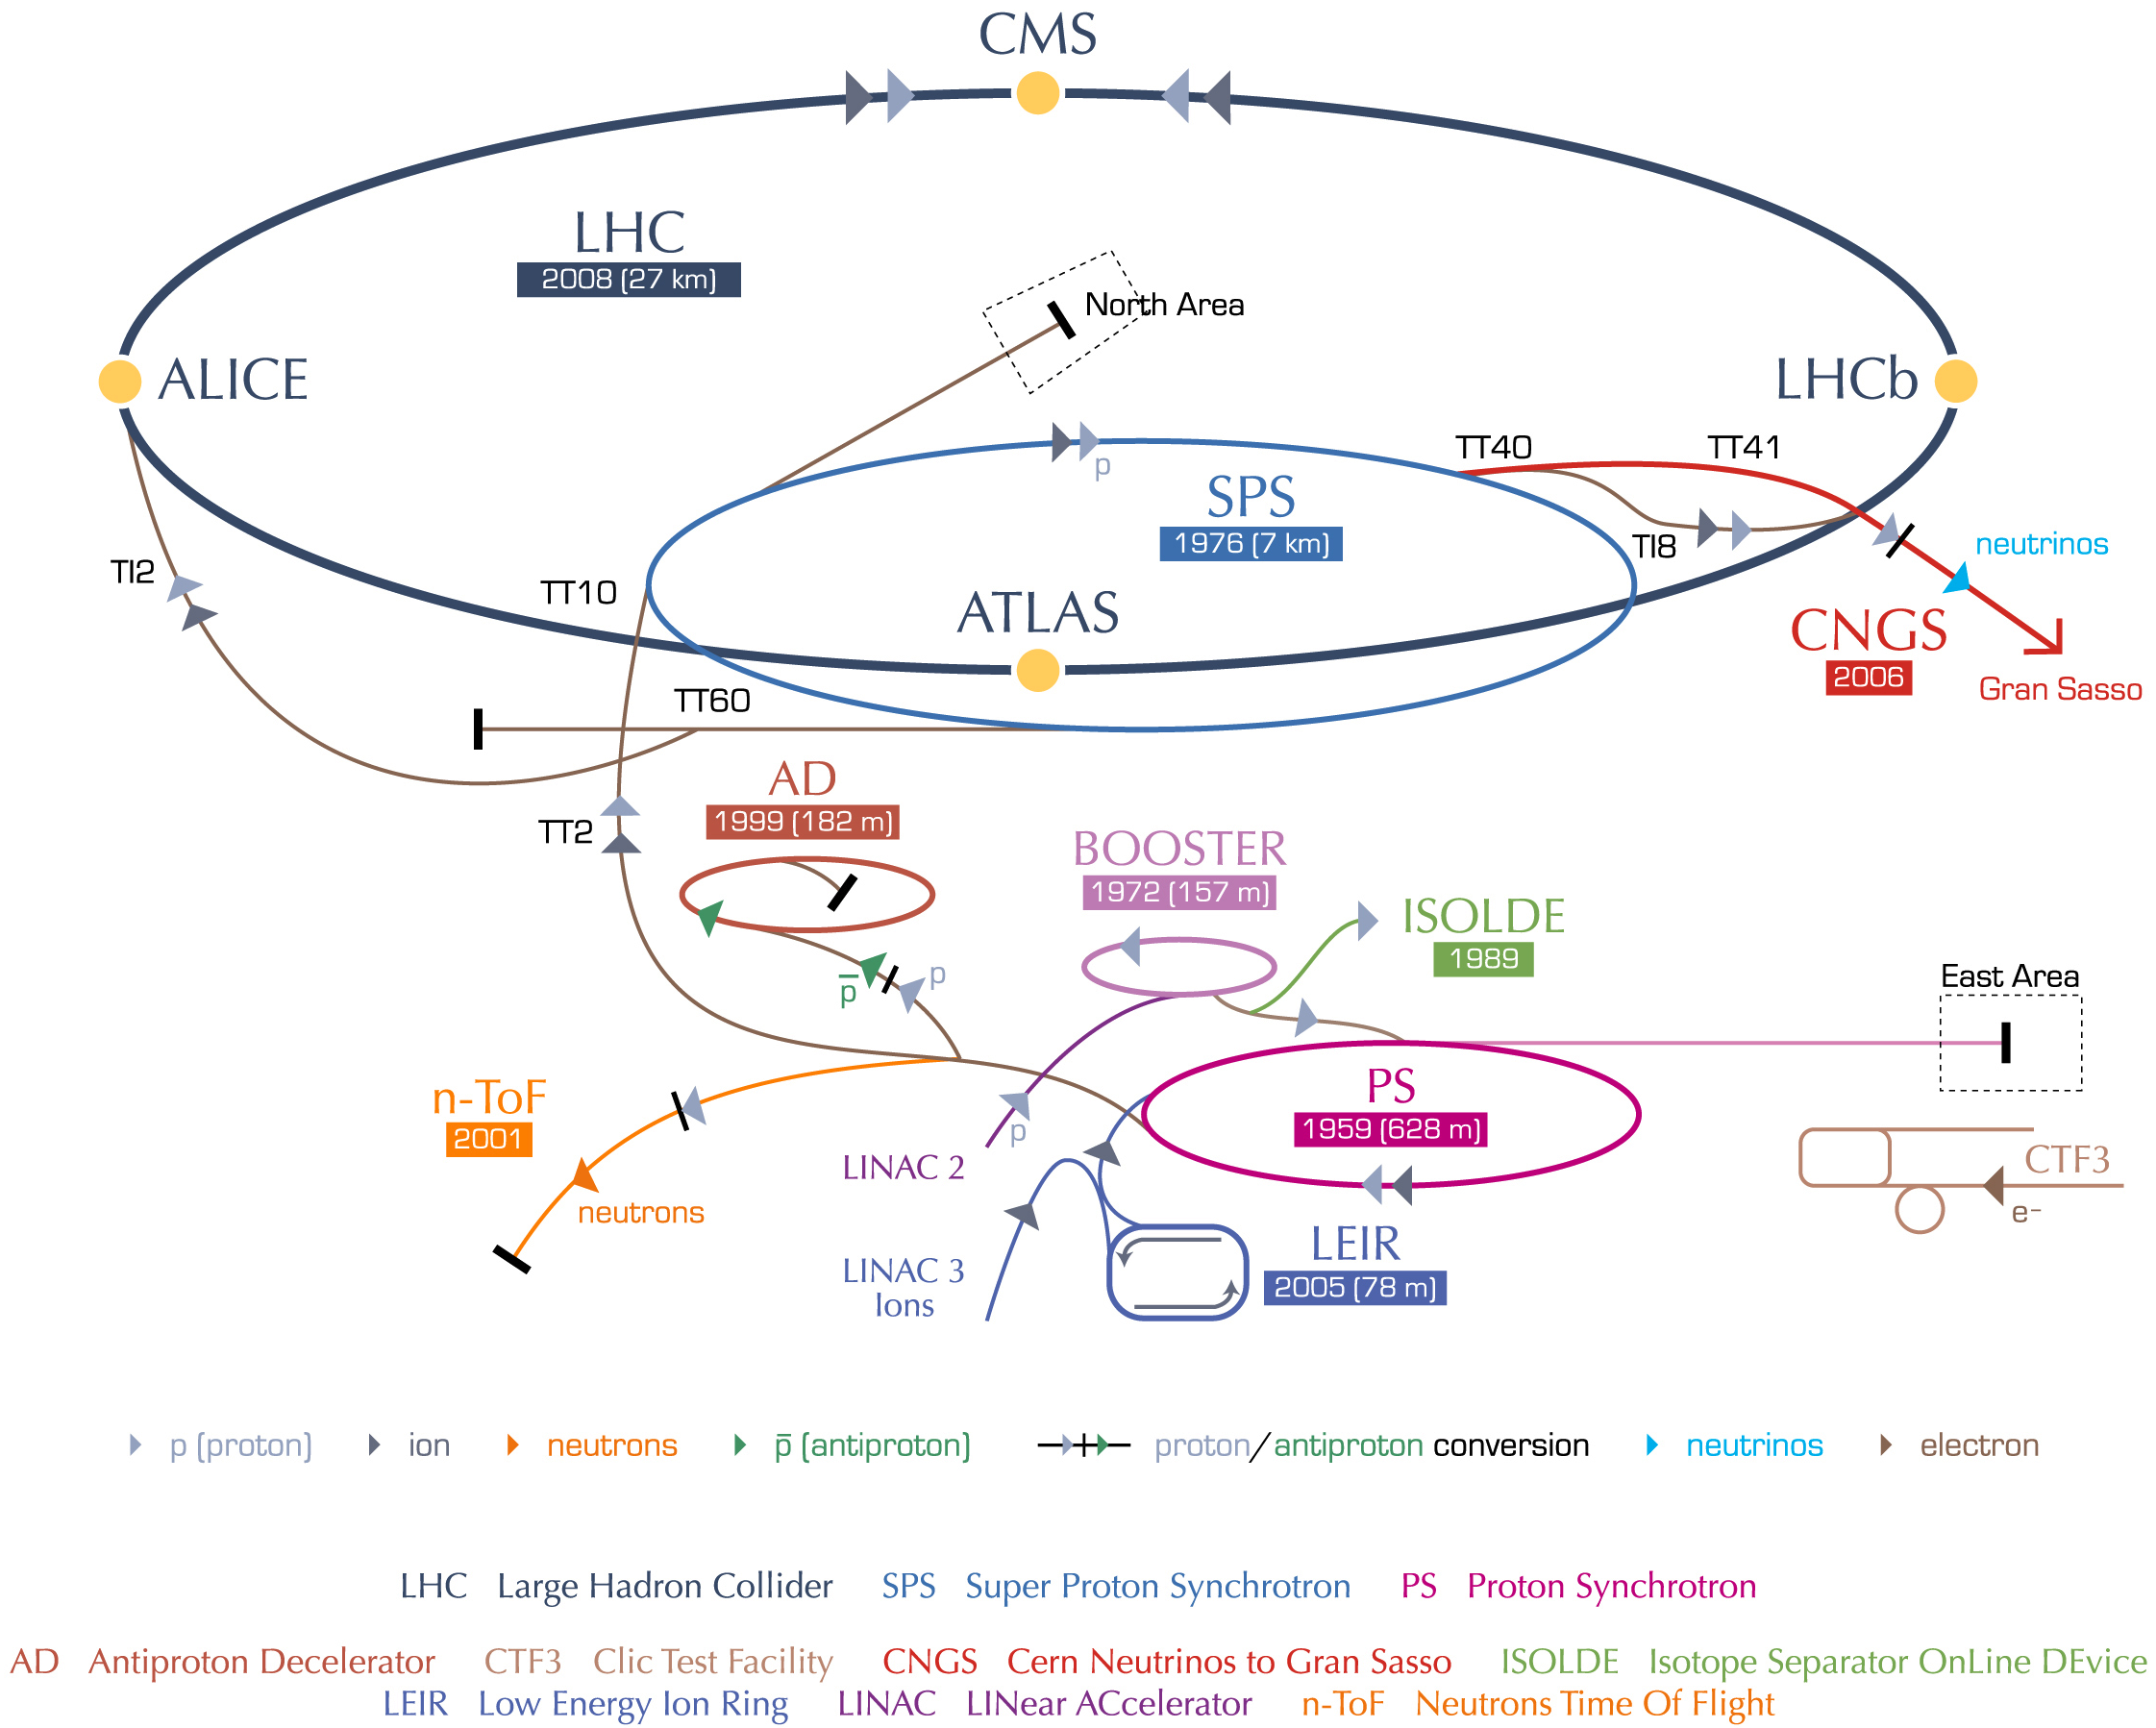
\includegraphics[width=\textwidth]{figures/cern-accelerator-complex-detail.png}
  \caption{Overview of the CERN accelerator complex.}
  \label{fig:lhc-complex}
\end{figure*}

The actual LHC ring consists of a pair of evacuated beampipes which pass through a series of bending and focusing magnets as well as RF cavities which boost and maintain the proton kinetic energy.  The magnets' unique twin-bore design produces oppositely-directed fields for the two counter-rotating beams of protons within a single structure, designed to provide the bending field of \SI{8}{T} necessary to confine a \SI{7}{TeV} proton beam in a ring of radius \SI{4.3}{km}.  While current technical difficulties have limited the achieved beam energy to \SI{4.0}{\TeV}, upgrades over the next several years are expected to bring the LHC magnets much closer to their design capacity.  A cryogenic system allows the magnets to avoid resistive losses by cooling them below \SI{2}{K} with liquid helium, bringing them into the superconducting regime.

\section{The Compact Muon Solenoid Experiment}
The analysis presented in this thesis relies on data collected with the Compact Muon Solenoid (CMS)~\cite{CMSPaper}, one of two general-purpose detectors installed in the LHC.  It has a broad physics reach as a result of a layered design with multiple calorimeter and tracking detectors arranged to complement one another and provide a nuanced view of collision events.  CMS earns its ``compact'' moniker by virtue of a novel design which fits both the electromagnetic and hadronic calorimeters inside of its solenoidal magnet, a goal which eluded the previous generation of detectors for hadron colliders. 
This design reduces energy loss and scattering for electrons and similarly energy loss for the converted photon allowing highly precise measurements of electrons and photons.
The arrangement of the subsystems can be seen in Figure~\ref{fig:cms-cutaway}.

The CMS design achieves hermetic coverage over a large solid angle by fitting endcaps on either side of a central barrel.  In most subsystems, there is sufficient overlap between the barrel and endcap such that particles can be well measured throughout the entire detector volume.

\begin{figure*}[htbp]
\centering
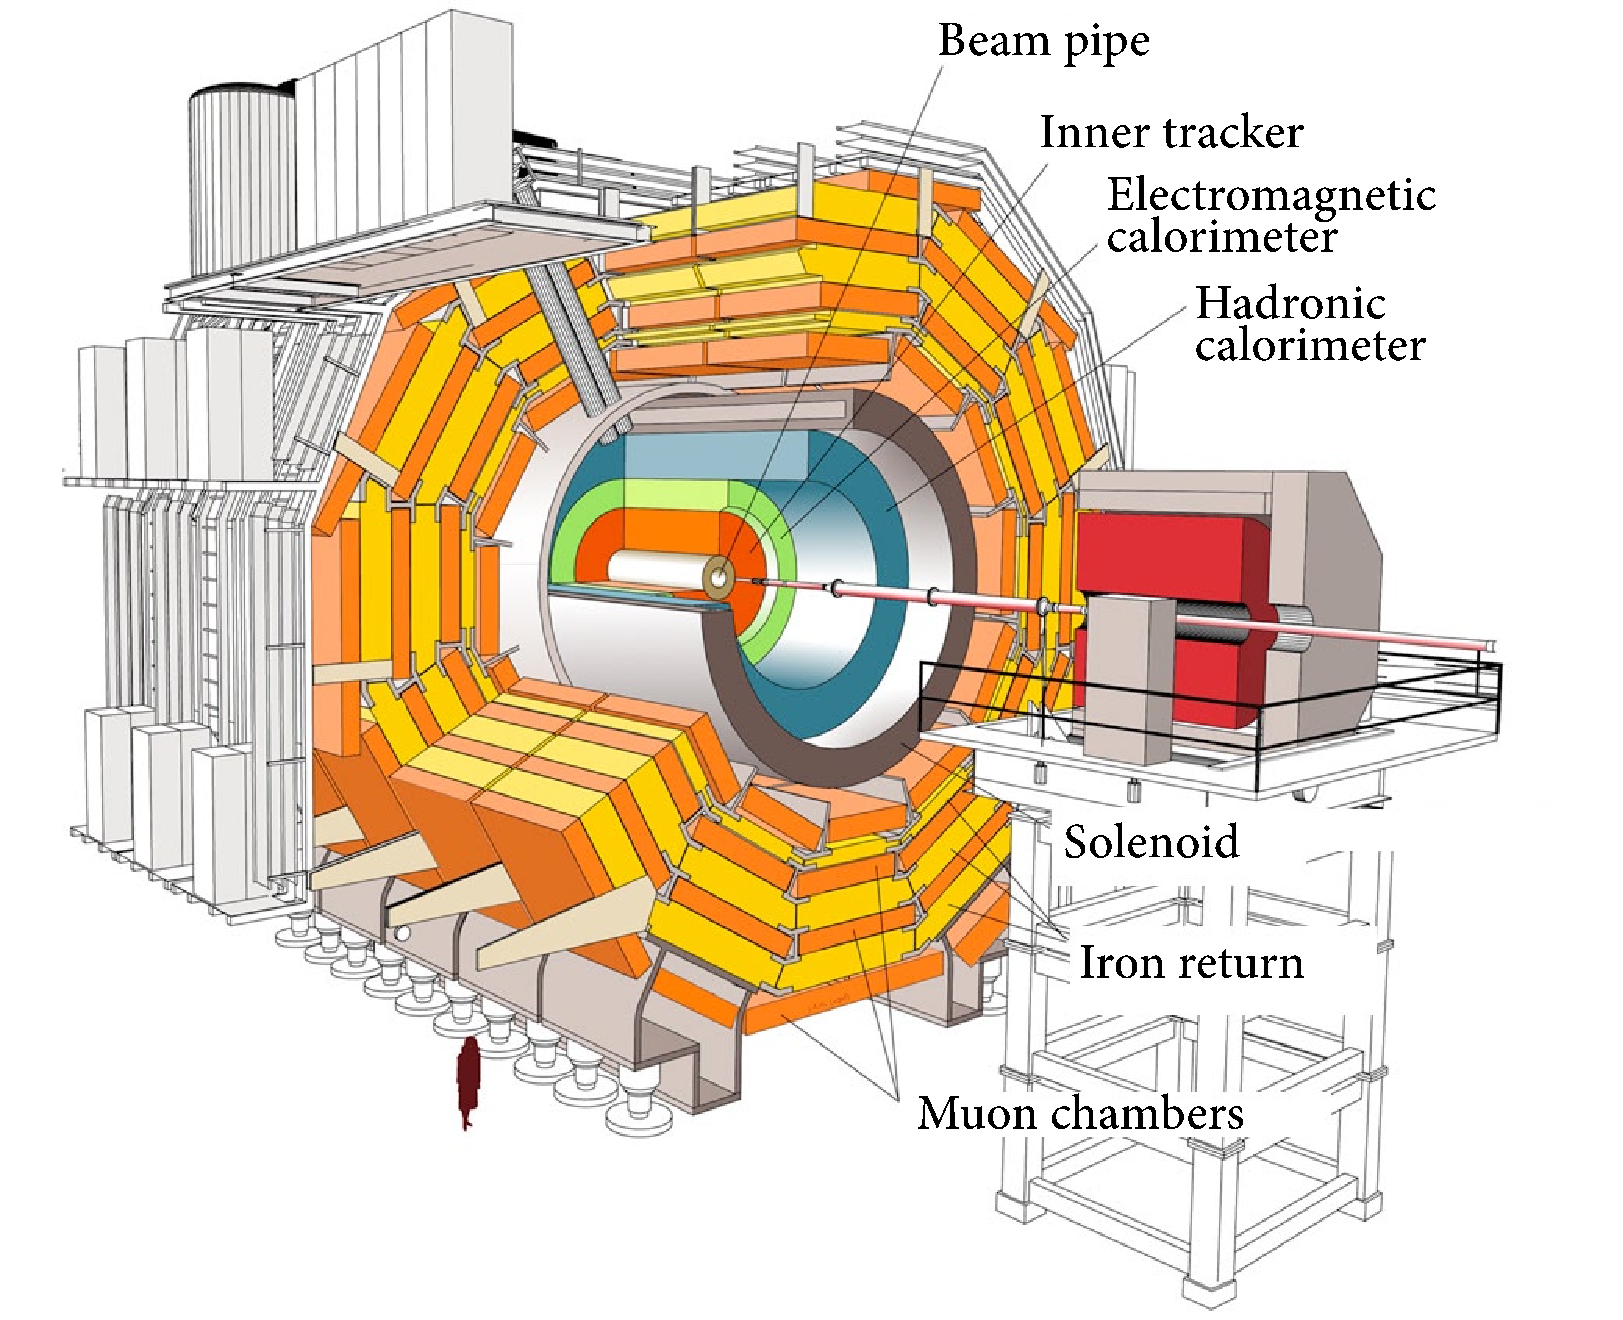
\includegraphics[width=4.5in]{figures/cms-cutaway.pdf}
\caption{A cut-away view of the barrel portion of the CMS detector with each of the main components labeled.}
\label{fig:cms-cutaway}
\end{figure*}

\subsection{Coordinate System}

% \begin{figure*}[!htbp]
%   \centering
%   \subbottom[Transverse view]{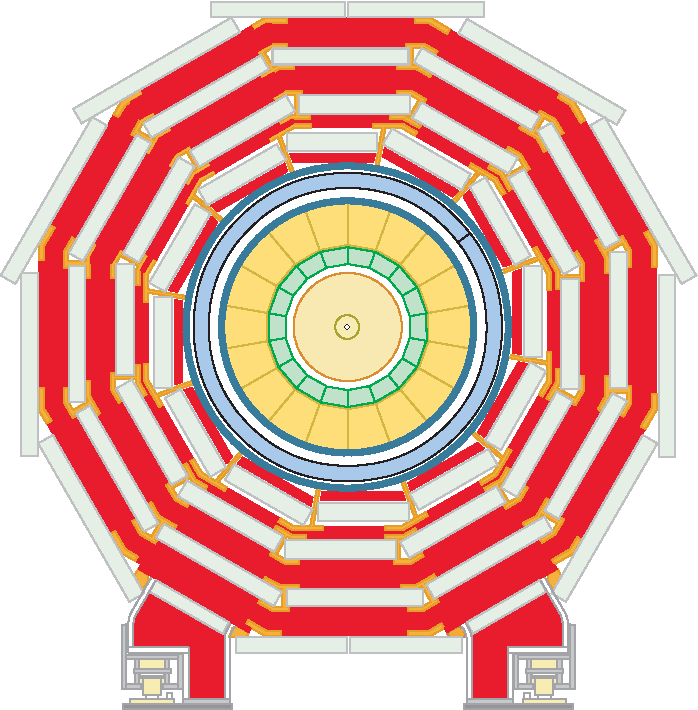
\includegraphics[width=0.35\textwidth]{figures/cms-xsection-trans.pdf}\label{cms-xsection-trans}}
%   \subbottom[Longitudinal view]{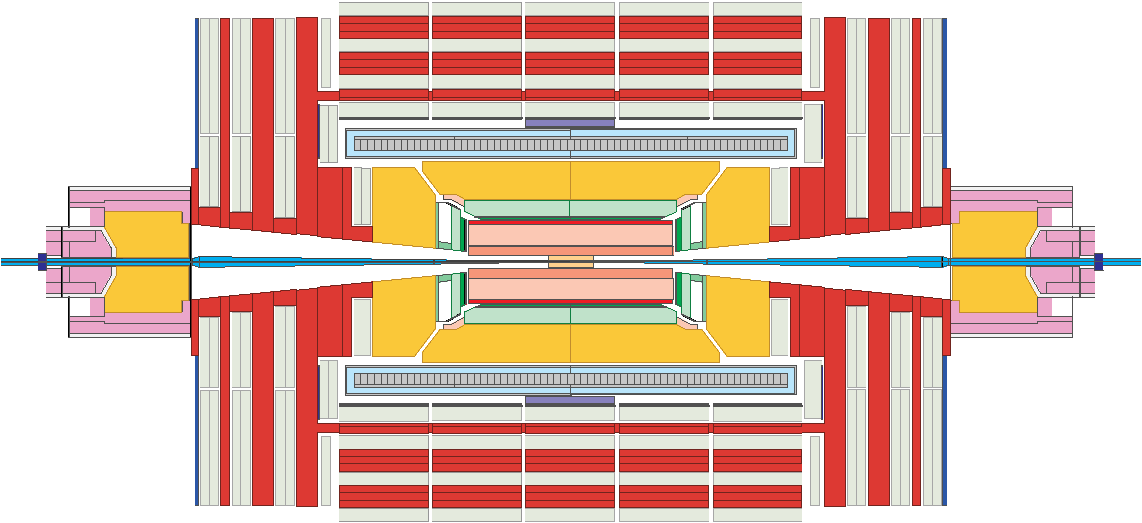
\includegraphics[width=0.65\textwidth]{figures/cms-xsection-long.pdf}\label{cms-xsection-long}}
%   \caption{Two cross-sectional views of the \cms detector.}
%   \label{cms-xsections}
% \end{figure*}

\begin{figure*}
  \centering
  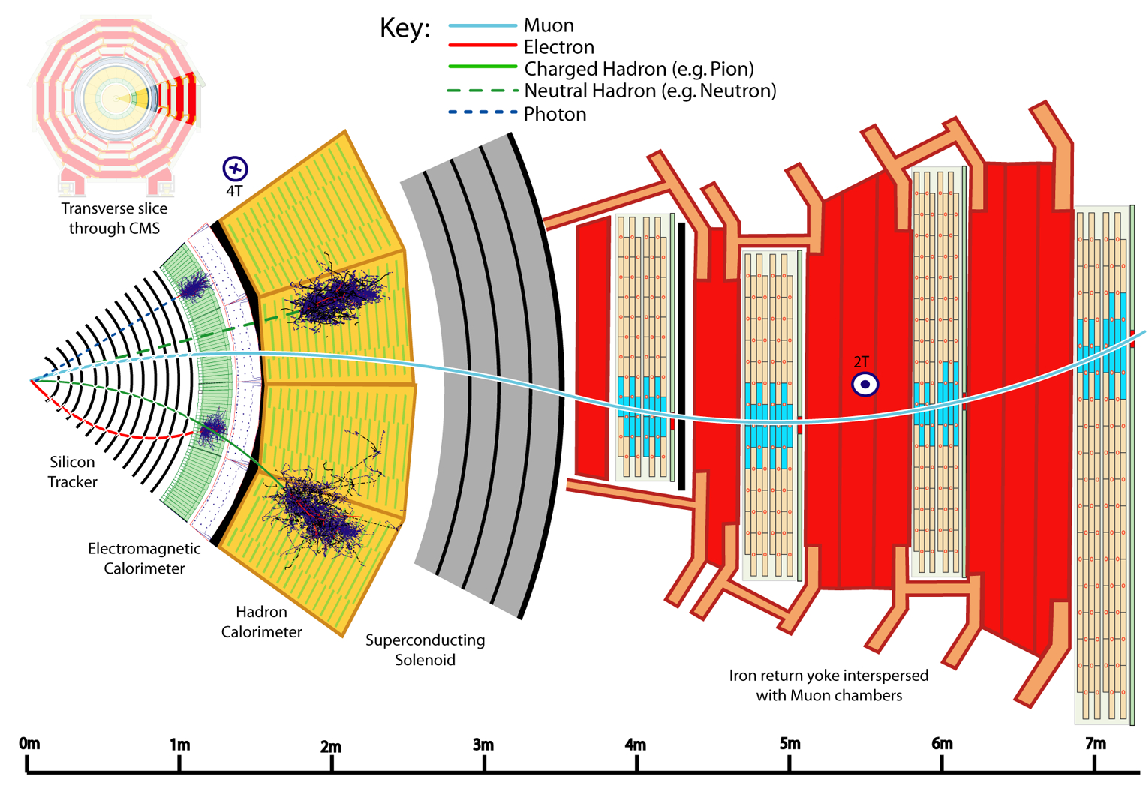
\includegraphics[width=\textwidth]{figures/cms-slice}
  \caption{A transverse slice of the CMS detector, showing the various subsystems and expected behavior of muons, electrons, photons, and hadrons.}
  \label{cms-xsections}
\end{figure*}

A location within the \cms detector can be described using a typical right-handed cartesian coordinate system originating from the center of the detector.  The $x-y$ plane forms a vertical cross section with the $y$-axis pointing upward and the $x$-axis pointing south toward the center of the LHC ring.  The $z$-axis points west, following the direction of the counter-clockwise proton beam as viewed from above.  Particles produced in collision events originate near the center of the detector and move quickly outward in all directions; for our measurements, then, we typically are concerned with the angle of the particle's initial trajectory away from the center of the detector.  To this end, we define the azimuthal angle $\phi = \arctan(y/x)$ and the polar angle $\theta = \arctan(\sqrt{x^2 + y^2}/z)$.

The products of 2-to-2 collisions mediated by the strong force, accounting for the vast majority of events produced by the LHC, tend to have momenta much larger along the $z$-axis than transverse to it, rendering the polar angle an inconvenient description for deviation from the beam pipe.  Particle physicists have traditionally defined a \emph{rapidity} relative to the beam axis,
\begin{equation}
  y \equiv \frac{1}{2}\ln\left(\frac{E + p_z}{E - p_z}\right),
\end{equation}
which in the relativistic limit ($E \approx |\vec{p}|$) reduces to a simple function of the polar angle,
\begin{equation}
  \label{eq:pseudorapidity}
  \eta = - \ln\left(\tan{\theta \over 2}\right).
\end{equation}
This quantity (known as \emph{pseudorapidity}) proves most convenient for describing deflection from the beam axis because the occupancy of the detector is approximately constant in equal $\eta$ intervals.  One of the distinguishing features of interactions that produce massive particles is that the decay products tend to be produced in a more spherical distribution, motivating a detector design with the best instrumentation in the central region of pseudorapidity.

\subsection{Solenoidal Magnet}
Much of the CMS design is driven by the desire to provide precise momentum measurements in the \TeV regime.  For a particle of charge $q$, the transverse momentum can be inferred from the radius of curvature of its trajectory ($r$) when it moves through a magnetic field $B$:
\begin{equation}
  \label{eq:curvature}
  \pt = q r B.
\end{equation}
The resolution of the radius measurement depends on the amount of curvature, so as particles move towards higher energies, the momentum resolution degrades.  In order to provide sufficient bending even for \TeV-scale particles, CMS was designed with the most powerful magnet built to date, sustaining a homogenous \SI{3.8}{T} magnetic field over a volume of more than \SI{300}{m^3}.  The return field saturates the iron yoke, providing a consistent \SI{2}{T} field throughout the outer muon system, allowing an additional, large lever arm measurement of the transverse momentum for highly penetrating particles such as muons.  The capabilities and geometry of the magnet guide the design of each of the CMS subsystems.

\subsection{Inner Tracker}

Starting from the beampipe and moving outward into CMS, the first instrumented region is the inner tracking detector.  The entire inner tracker is based on a silicon semiconductor design.  As charged particles traverse the tracker, they deposit ionization energy, dislodging electrons which in turn produce secondary ionization.  The semiconducting silicon is held at a high voltage, causing the released electrons and corresponding holes to separate.  The electrons are collected as an electric pulse, with some threshold applied to indicate a ``hit'', or the passage of a charged particle through a particular region of silicon. 

The primary role of the inner tracker is to provide precise measurements of the trajectories of all charged particles.  Its resolution, however, is also sufficient to distinguish a secondary vertex in a single collision event corresponding to displaced tracks which are the hallmark of the relatively short-lived hadrons containing $b$ or $c$ quarks; this allows discrimination between prompt leptons produced from the decay of vector bosons and secondary leptons produced in the semileptonic decays of hadrons.  The total tracker system, \SI{5.8}{m} in length and \SI{2.5}{m} in diameter, consists of silicon pixels and strips, arranged in various layers, and covers the pseudorapidity region $-2.5<\eta<2.5$.

The first three layers (out to a radius of \SI{10.2}{cm}) consist of silicon pixels which provide maximum precision and granularity for the extremely high particle occupancies expected in a region so close to the interaction point~\cite{Kastli2007724}.  Each of the approximately 66 million pixels is $\SI{100}{\micro m} \times \SI{150}{\micro m}$ in size, leading to a total coverage of \SI{1}{m^2}.  The pixels provide tracking points in both the $r-\phi$ (resolution $~\SI{10}{\micro m}$) and $r-z$ (resolution $~\SI{20}{\micro m}$) planes.  The design's emphasis on providing a $z$ resolution on par with the $r-\phi$ resolution is the key feature which allows successful secondary vertex reconstruction in three dimensions.

\begin{figure*}
  \centering
  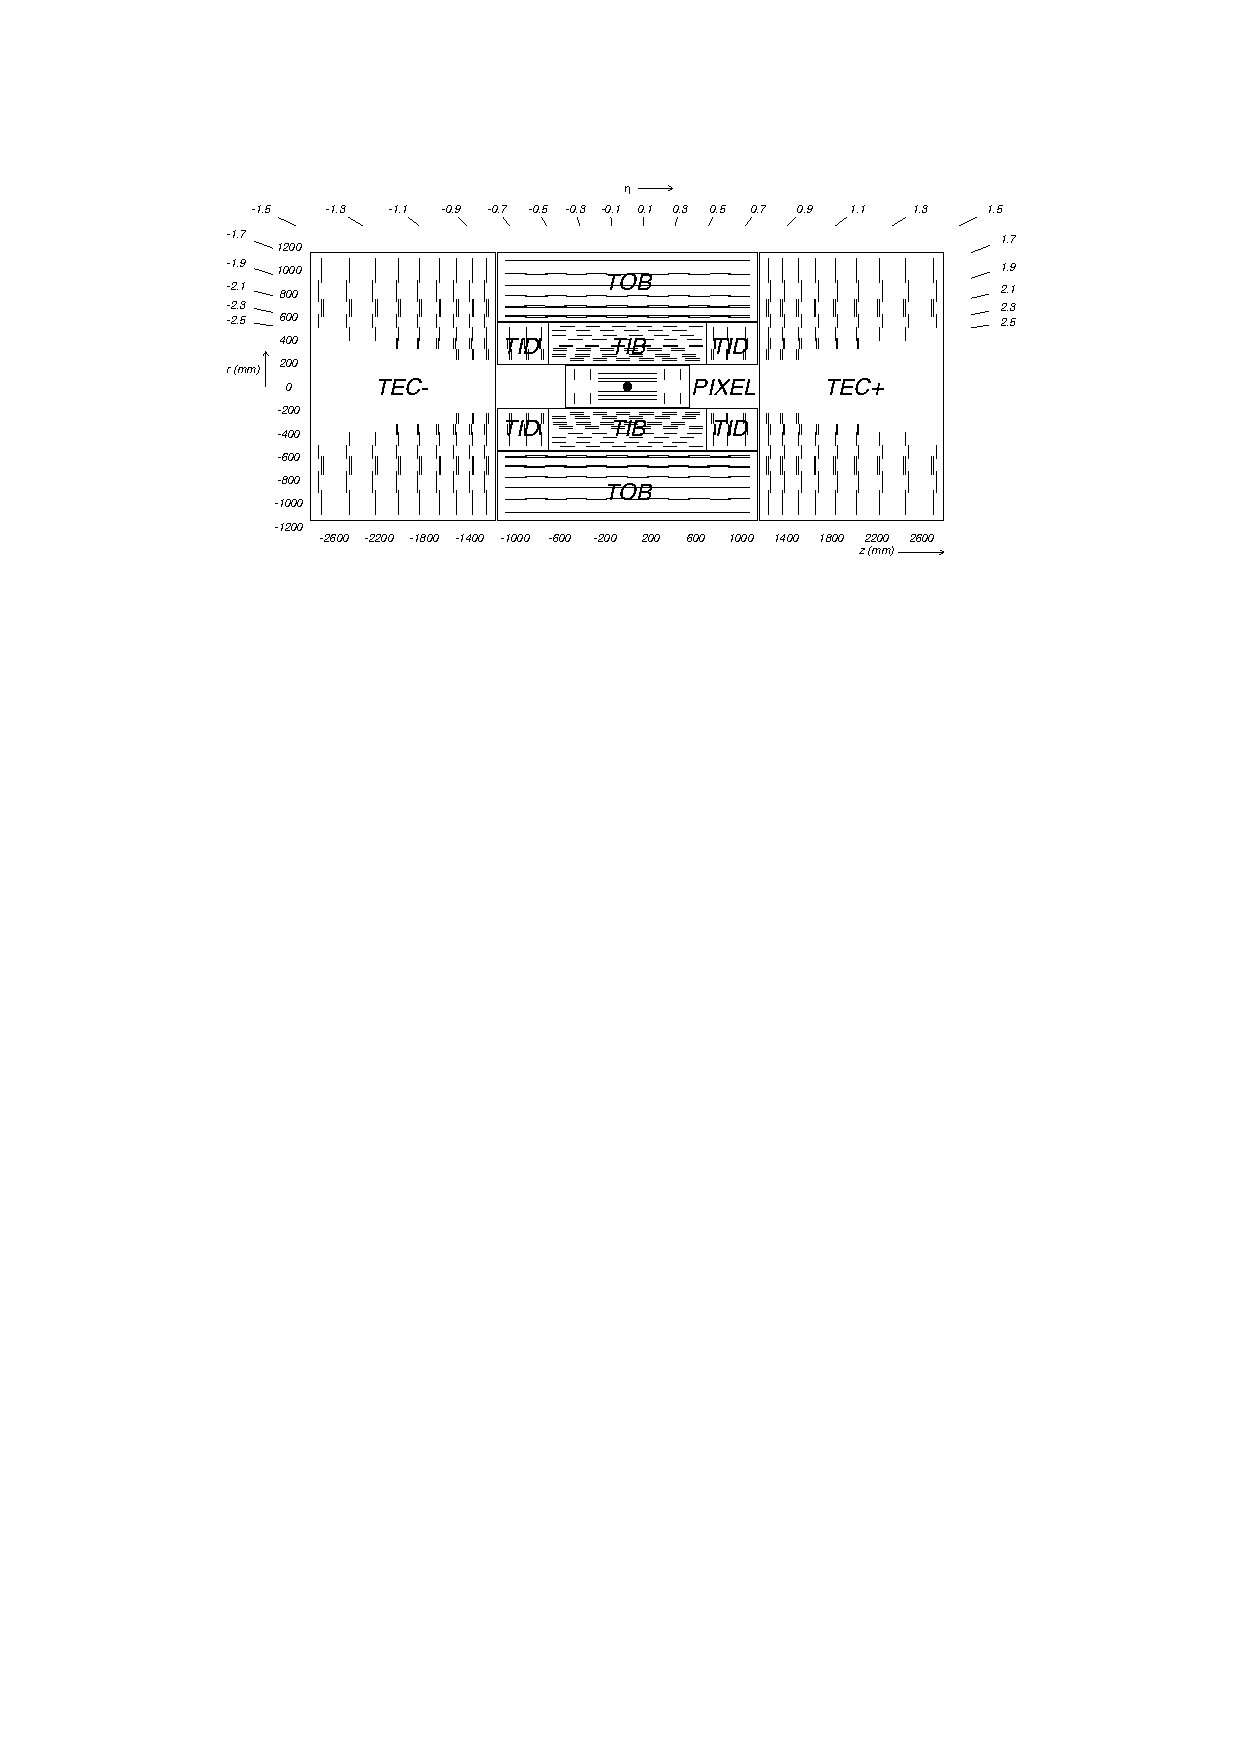
\includegraphics[width=\textwidth]{figures/cms-tracker-xsec.pdf}
  \caption[Schematic cross section through the CMS tracker]{Schematic cross section through the CMS tracker.  Each line represents a detector module.  Double lines indicate back-to-back modules which deliver stereo hits~\cite{Evans:1129806}.}
  \label{fig:tracker-xsec}
\end{figure*}

Outside the pixel system lie ten layers of silicon microstrip detectors, each strip \SI{10}{cm} to \SI{25}{cm} long with a height of \SI{180}{\micro m} and spacing between the strips (known as ``strip pitch'') varying by region.  The strips are distributed across two barrel regions, the tracker inner barrel (TIB, strip pitch of \SI{80}{\micro m} to \SI{120}{\micro m}) and the tracker outer barrel (TOB, strip pitch of \SI{120}{\micro m} to \SI{190}{\micro m}), along with two endcap regions, the tracker inner disks (TID) and the tracker endcaps (TEC) with radial strips of \SI{97}{\micro m} to \SI{184}{\micro m} average pitch.  The overall layout of the tracker subsystems can be seen in Figure~\ref{fig:tracker-xsec}.

Hits in the silicon pixels and strips are used as input to reconstruction algorithms which connect them together into tracks and calculate the associated momenta.  The momentum resolution of the tracker is 
\begin{equation}
  %\frac{\sigma(\pt)}{\pt} = \frac{\pt}{\GeV} \cdot 0.015\% \oplus 0.5\%
  \frac{\sigma(\pt)}{\pt} = (\pt/\GeVc) \cdot 0.015\% \oplus 0.5\%
\end{equation}
for $|\eta| < 1.6$, with the relative error increasing in the forward region to a maximum of
\begin{equation}
  %\frac{\sigma(\pt)}{\pt} = \frac{\pt}{\GeV} \cdot 0.060\% \oplus 0.5\%
  \frac{\sigma(\pt)}{\pt} = (\pt/\GeVc) \cdot 0.060\% \oplus 0.5\%
\end{equation}
for $|\eta| = 2.5$.  The first term accounts for the curvature measurement which becomes less precise for high-momentum tracks that bend only slightly in the magnetic field.  The second term accounts for interactions with the tracker material such as multiple scattering.

\subsection{Electromagnetic Calorimeter}
\label{sec:ecal}

\begin{figure*}
  \centering
  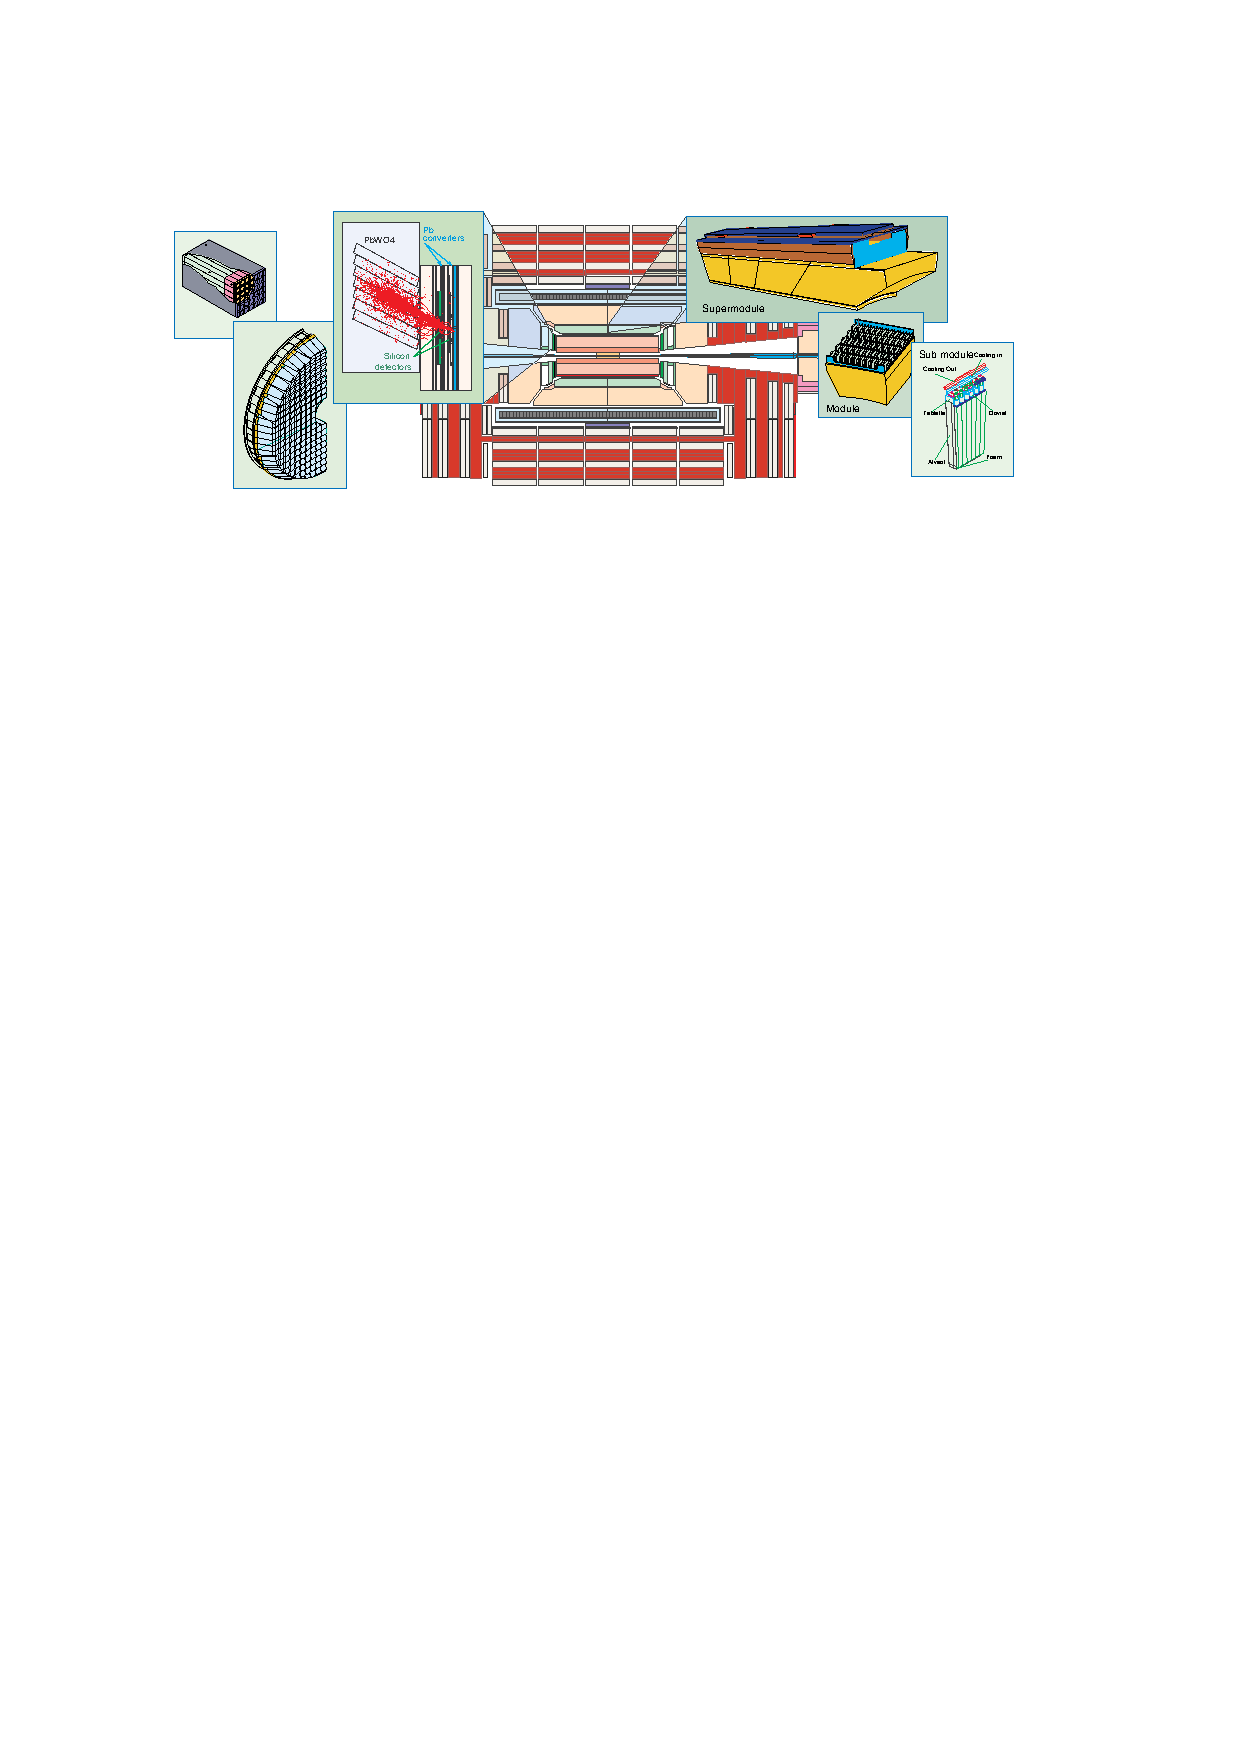
\includegraphics[width=\textwidth]{figures/cms-ecal}
  \caption{A schematic showing the various features of the CMS \ecal.}
  \label{fig:cms-ecal}
\end{figure*}

The CMS electromagnetic calorimeter (\ecal) is designed to detect electrons and photons, inducing electromagnetic showers and collecting the resultant photons.  The \ecal{} is able to achieve a remarkably high energy resolution due both to the homogenous coverage provided by a crystal-based design and to its location inside the solenoid, avoiding the significant degradation seen in previous hadron collider experiments due to interactions in the magnet material.  To keep the solenoid a reasonable size, however, the \ecal{} must be incredibly compact, necessitating a dense interaction material which maintains transparency under high doses of radiation so that photons can reach a collection region with minimal energy loss.  Lead tungstate (\leadtungstate) crystals provide a high density (\SI{8.28}{g/cm^3}), short radiation length (\SI{0.89}{cm}), and small Moli\`{e}re radius (\SI{2.2}{cm}), leading to rapidly progressing, tightly contained showers for high-energy electrons and photons.  The crystals emit a blue-green scintillation light peaking near \SI{425}{nm}, which is collected by avalanche photodiodes (APDs) and vacuum phototriodes (VPTs).  The APDs and VPTs produce electrical signals which correlate with the multiplicity of detected photons, allowing us to calculate ``energy deposits'' left in each crystal.  A schematic is provided in Fig.~\ref{fig:cms-ecal}.

The \ecal barrel (EB) offers pseudorapidity coverage to $|\eta| < 1.479$ through use of \num{61200} crystals, each with a tapered shape of roughly $\SI{22}{mm} \times \SI{22}{mm}$ at the front face, widening to $\SI{26}{mm} \times \SI{26}{mm}$ at the rear, and with a \SI{230}{mm} length of which provides approximately 26 radiation lengths of material. The precise shape of the crystals is slightly different in various $\eta$ regions.  The EB crystals are arranged into modules ($~500$ crystals) and supermodules (1700 crystals) which various structural and readout elements.

The \ecal endcaps (EE) cover a pseudorapidity range $1.479 < |\eta| < 3.0$ through use of \num{14648} identically-shaped crystals, again with a tapered design widening from $\SI{28.62}{mm} \times \SI{28.62}{mm}$ at the front face to $\SI{30}{mm} \times \SI{30}{mm}$ at the rear, with a \SI{220}{mm} length corresponding to 25 radiation lengths.  They are grouped into $5 \times 5$ mechanical units called supercrystals.

Energy deposits in individual crystals are combined into clusters of energy, which are further grouped into superclusters in the reconstruction algorithms, serving as the starting point for identification of electrons and photons in the detector.  The \ecal achieves an energy resolution given as:
\begin{equation}
  \frac{\sigma(E)}{E} = \frac{1}{\sqrt{E/\GeV}} \cdot 2.8\% \oplus \frac{1}{E/\GeV} \cdot 0.0415\% \oplus 0.3\%
\end{equation}
where the three terms correspond to statistical fluctuations and intrinsic shower fluctuations; electronic noise and pileup energy; and detector non-uniformity and calibration uncertainties.

\subsection{Hadronic Calorimeter}

\begin{figure*}
  \centering
  \includegraphics[width=\textwidth]{figures/cms-hcal}
  \caption{A schematic showing the various features of the CMS \hcal.}
  \label{fig:cms-hcal}
\end{figure*}

The CMS hadronic calorimeter (\hcal) is designed to detect particles which primarily interact with atomic nuclei via the strong force.  Measurement of the energy of such particles is particularly import for the reconstruction of jets of hadrons and missing transverse energy, which could indicate the presence of neutrinos or long-lived neutral exotic particles in collision events.  Strongly interacting particles typically start showering in the dense material of the \ecal{}, so a full picture of a jet's energy relies combining information from both the electromagnetic and hadronic calorimeters.  

The basic design of the \hcal is a sampling calorimeter with alternating layers of brass and scintillator.  The brass acts as a non-ferromagnetic absorber, capable of withstanding the intense magnetic field, providing \num{5.82} interaction lengths of material in the barrel to encourage development of hadronic showers.  The scintillator consists of tiles along with wavelength-shifting fibre.  Hadrons interact with the scintillating material to produce a broad spectrum of photons which are then absorbed in the fibre and re-emitted in a more narrow range to which the photodetectors are sensitive.  In the endcap, brass is replaced with steel and tile with quartz, which are both better able to withstand the higher radiation dose in that region.  A schematic is provided in Fig.~\ref{fig:cms-hcal}.

The resolution for the barrel and endcap \hcal ($|\eta| < 3.0$) is given as:
\begin{equation}
  \frac{\sigma(E)}{E} = \frac{1}{\sqrt{E/\GeV}} \cdot 85\% \oplus 7.4\%
\end{equation}
with stochastic and constant terms in analogy to those discussed for the \ecal.  The inferior performance relative to the \ecal is due both to its operating principle of sampling the shower rather than absorbing all produced energy in high-resolution crystals and also to the intrinsically lower particle multiplicity in hadronic showers vs.\ electromagnetic showers, leading to wider statistical fluctuations.

\subsection{Muon System}

\begin{figure*}
  \centering
  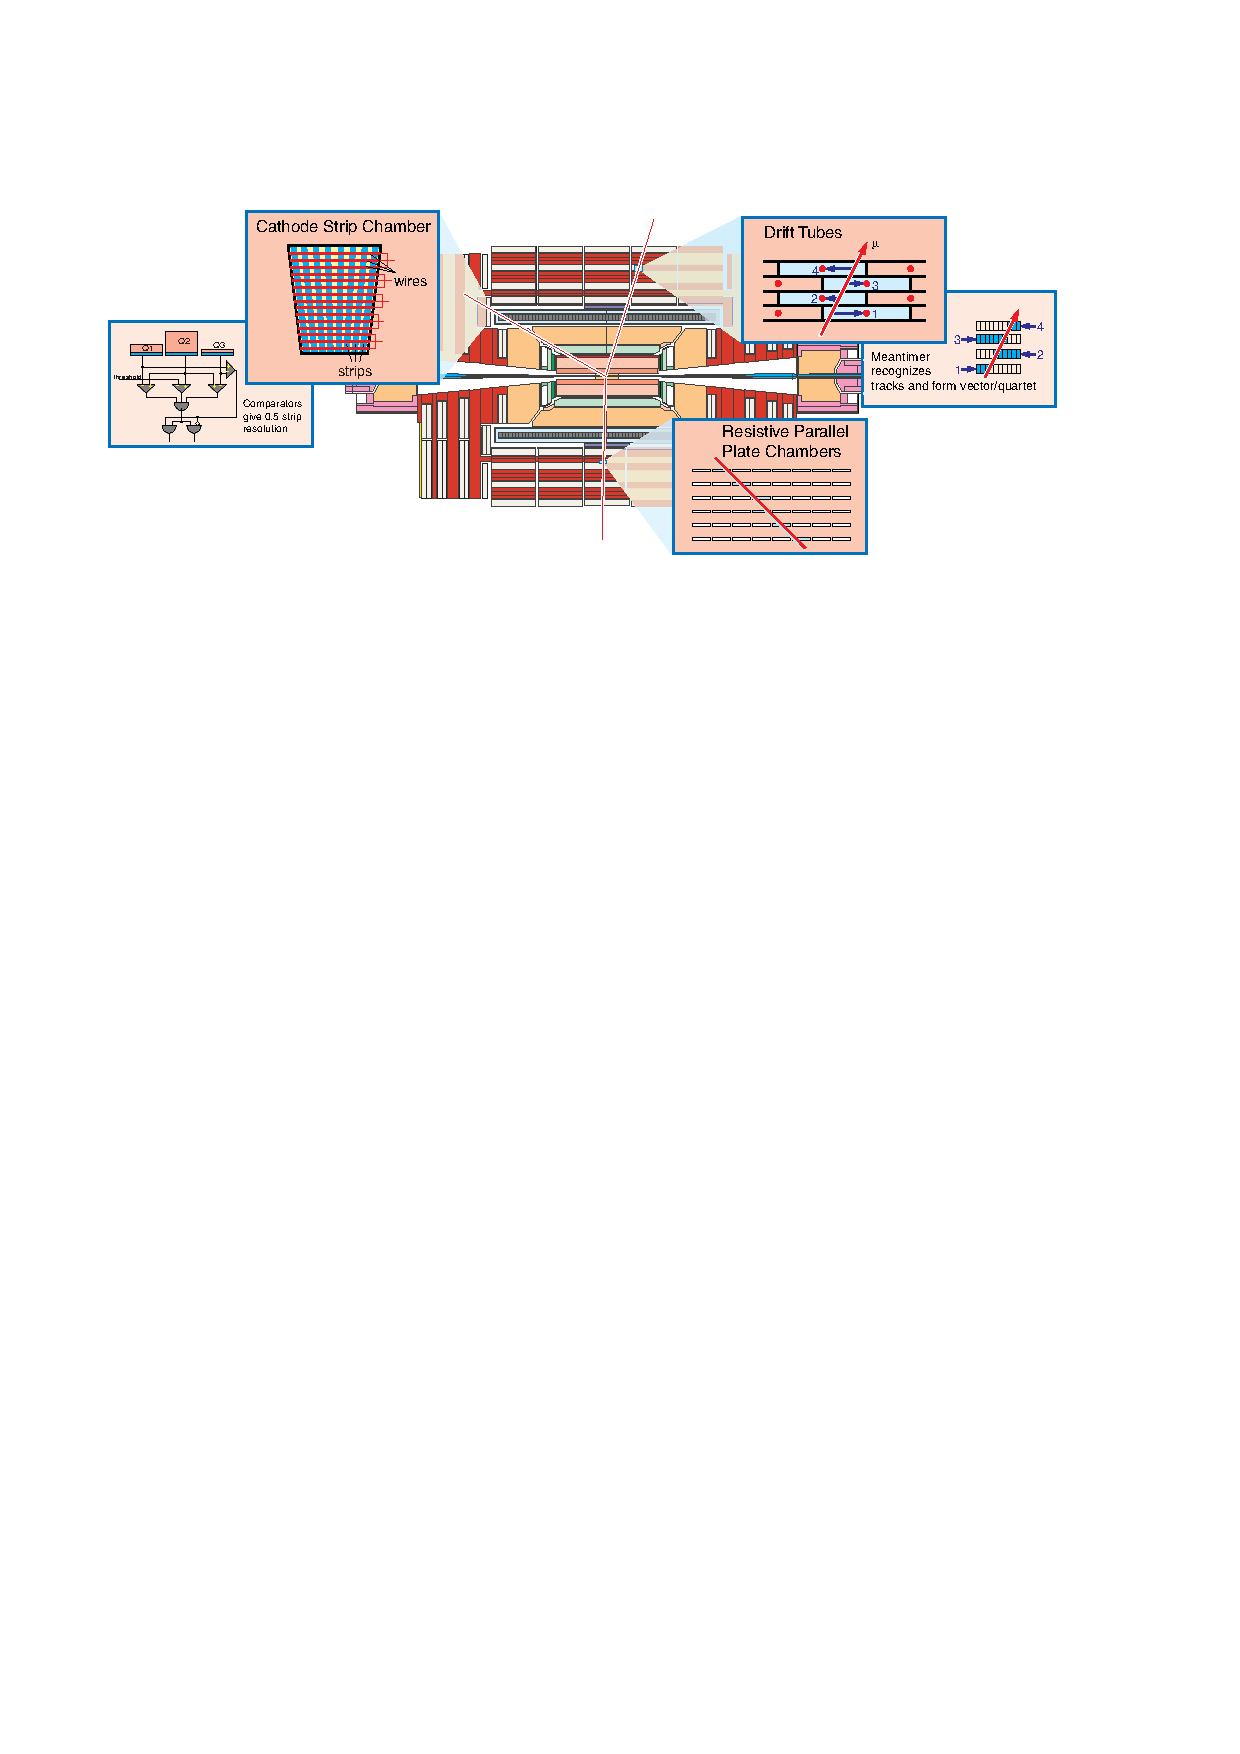
\includegraphics[width=\textwidth]{figures/cms-muon-system}
  \caption{A schematic overview of the various muon detector technologies.}
  \label{fig:cms-muon-system}
\end{figure*}

As suggested by its name, the Compact Muon Solenoid is designed with the detection of muons as a high priority.  As such, it includes an advanced muon spectrometer capable of distinguishing muons with high accuracy and contributing to an impressive momentum resolution for energetic muons.  The muon system employs three types of gaseous particle detectors optimized for different environments and goals -- drift tubes (DTs) in the barrel, cathode strip chambers (CSCs) in the endcaps, and resistive plate chambers (RPCs) covering nearly the entire barrel and endcap regions.

Muon chambers are arranged in 4 stations embedded in a heavy iron yoke with each consecutive station located further from the interaction region.  The iron yoke provides a support structure for the various chambers and concentrates the return field of the solenoid in order to provide significant bending of muons for the momentum measurement.  A schematic showing the layout of the muon system is provided in Fig.~\ref{fig:cms-muon-system}.

DTs consist of chambers filled with a gas mixture ionized by the passage of charged particles.  Within each chamber is a wire held at high voltage, setting up an attracting electric field to collect the ionization charge, producing an electric pulse in the wire indicating the presence of a particle.  Because the drift velocity for electrons in a particular gas mixture is well defined, a drift tube can provide a precise measurement of the particle's position based on the drift time of the collected charge. These chambers are an economical and robust choice as the primary muon system detector in the CMS barrel, a region with low occupancy and modest magnetic field, but they have a relatively slow response (drift time up to \SI{380}{ns}) which disqualifies them for use in the more active endcap region.  The sensitive wires in each tube are \SI{2.4}{m} long and the gas is a mixture of argon and carbon dioxide.  Each DT chamber consists of three superlayers, each composed in turn of four layers of rectangular drift cells staggered by half a cell.  The two outer superlayers are oriented with the wires parallel to the beam to provide tracking in the $r-\phi$ plane in which the muon bends due to the magnetic field.  The third superlayer, present only in the first three stations, measures the $z$ coordinate.

The higher occupancy of the endcap regions requires the fast performance and high granularity of CSCs.  The CSC is a type of multiwire proportional chamber where a plane of multiple anode wires is housed within a single gas chamber, with each wire acting as an individual proportional counter.  The wires are held at voltage, providing an electric field such that the electrons produced by ionization due to a passing charged particle are drawn to the wires, producing an electric signal indicating the particle's presence.  The CMS endcaps contain a total of 468 CSCs, each comprised of six anode wire planes interleaved among 7 cathode panels.  All wires run azimuthally, with the $\phi$ coordinate localized by interpolating charges induced on the strips.  

An RPC~\cite{Santonico1981377} consists of parallel electrode plates, setting up a constant and uniform electric field across an ionizing gas in the gap.  The electrodes are constructed with a high resistivity such that the electric field is suddenly switched off when a charged particle causes an ionization discharge in the gas, preventing the charge from propagating through the gas.  The uniform field design yields a much better time resolution than wire chambers with a $1/r$ field dependence around each wire.  The RPCs installed in the CMS muon system employ a double-gap design operating in avalanche mode and although they cannot compete with either the DTs or the CSCs for spatial resolution, their superior timing resolution is fine enough to unambiguously associate muon hits to a particular bunch crossing, even with the high rate and pileup of the full LHC luminosity.  As such, they are useful in triggering muon events.

\subsection{Trigger System}

At design luminosity of the LHC, we expect beam crossings at a frequency of \SI{40}{MHz} leading to collisions on the order of one billion per second delivered to CMS, allowing unprecedented access to rare physics events.  Ideally, we would like to be able to keep a record of every delivered collision, but no data acquisition or storage system available with current technology would be able to deal with even a hundredth of the requisite rate.  Most events at the LHC, however, consist only of ``soft'' collisions without a significant momentum transfer, producing final states with low-energy jets which have been extensively studied at lower-energy colliders and are unlikely to reveal new physics insights.  By ignoring these low-energy events, we can define a more tractable stream of collisions with higher likelihood for interesting content.  Determining which events to keep, however, requires a specialized ``trigger'' system capable of making sub-millisecond decisions about the physics potential of incoming events.

The CMS trigger system uses custom hardware combined with a computing farm to achieve a million-fold reduction in the stored event rate.  The hardware step, called the level-1 (L1) trigger, is designed with an output rate of \SI{100}{kHz}, using coarsely binned information from the detector to quickly detect any potentially interesting physics content in an event.  Events selected by L1 are passed to the high-level trigger (HLT), where commercial computing nodes run speed-optimized reconstruction algorithms in order to further reduce the event rate to a target of \SI{300}{Hz} to \SI{400}{Hz} for permanent storage.

\subsection{Luminosity Measurement}

The LHC machine cannot itself measure the luminosity of proton collisions, so the CMS detector itself must be used to perform a measurement, leading to one of the largest sources of error in cross section measurements and in new particle searches.  As a result, much attention has been paid to providing a reliable and precise luminosity measurement at CMS.  

Through 2011, CMS had been using a luminosity determination~\cite{LUMIPAS} based on activity in the forward hadronic calorimeter (HF) which covers the pseudorapidity range $3 < |\eta| < 5$ to record the transverse energy of forward jets.  The primary technique involves ``zero counting'' where the mean number of interactions per bunch crossing is inferred from the average fraction of empty calorimeter towers.  The technique requires calibration through a Van der Meer scan where the size and shape of the interaction region is measured by recording the relative interaction rate as a function of the transverse beam separations~\cite{vanderMeer:296752}.  This Van der Meer calculation includes a dependence on the LHC beam currents, which are only known to an accuracy of 3.1\%~\cite{Alice:1333997}, which becomes the primary contributor to the total uncertainty of 4.5\% on the luminosity measurement.

The new luminosity measurement approved in early 2012~\cite{CMS-PAS-SMP-12-008} relies on a calibration procedure based on cluster counting in the pixel tracker.  Because of the very fine granularity of the pixel tracker, the probability of a given pixel being hit by two different tracks in one bunch crossing is small, meaning that the number of clusters per crossing should vary linearly with the number of interactions per crossing and thus the luminosity.  This technique also requires a Van der Meer scan, but here the calibration involves monitoring pixel activity with less acute dependence on the LHC beam current, allowing a precise determination of the effective pixel cluster cross section.  That cross section is then applied to determine an instantaneous luminosity for each luminosity section (corresponding to \SI{23.3}{s} of collisions) of the 2011 physics data sample based on the level of activity in the pixels.  The new method achieves a total systematic uncertainty of 2.2\%.

